\begin{frame}
\begin{enumerate}
\item Hierarchy is a fundamental organizing concept in biology. 
\pause \item The existence of a number of apparently discrete levels of organization including molecules, cells, organisms, populations, communities, ecosystems, and more fine-grained levels below, above and in between these are taken for granted. 
\pause \item Theoretical constructs capable of integrating information about such levels of organization and of explaining the emergence of such levels in the evolutionary process have not been adapted to a biological context.
\end{enumerate}
\end{frame}

\begin{frame}
\begin{enumerate}
\item We can make use of existing theory to characterize coherence constraints that must ostensibly be satisfied in any evolutionary process in which at least two levels of organization become coupled such that one serves as a base supporting interactions among higher-level entities in another. 
\pause \item In this way, what may be considered as two distinct levels may come to be viewed as part of a unified system. 
\pause \item This process of unification of distinct levels may serve as a basis for induction in the consideration of arbitrarily complex compositions of multilevel biological systems.
\end{enumerate}
\end{frame}

\begin{frame}
\begin{enumerate}
\item The language we use to express these constraints is sufficiently general that it applies equally to several different concrete formalisms for representing biological systems
\pause \item For example, those that have become commonplace in the context of network science: algebraic graphs, hypergraphs, or (cell) complexes. 
\pause \item The derived relationship between levels of organization in models of biological systems can be used to constrain dynamical models defined in terms of transformations of graphs or another concrete relational structure that seek to take into account hierarchical transitions in evolutionary processes.
\end{enumerate}
\end{frame}

\begin{frame}
\begin{figure}
\noindent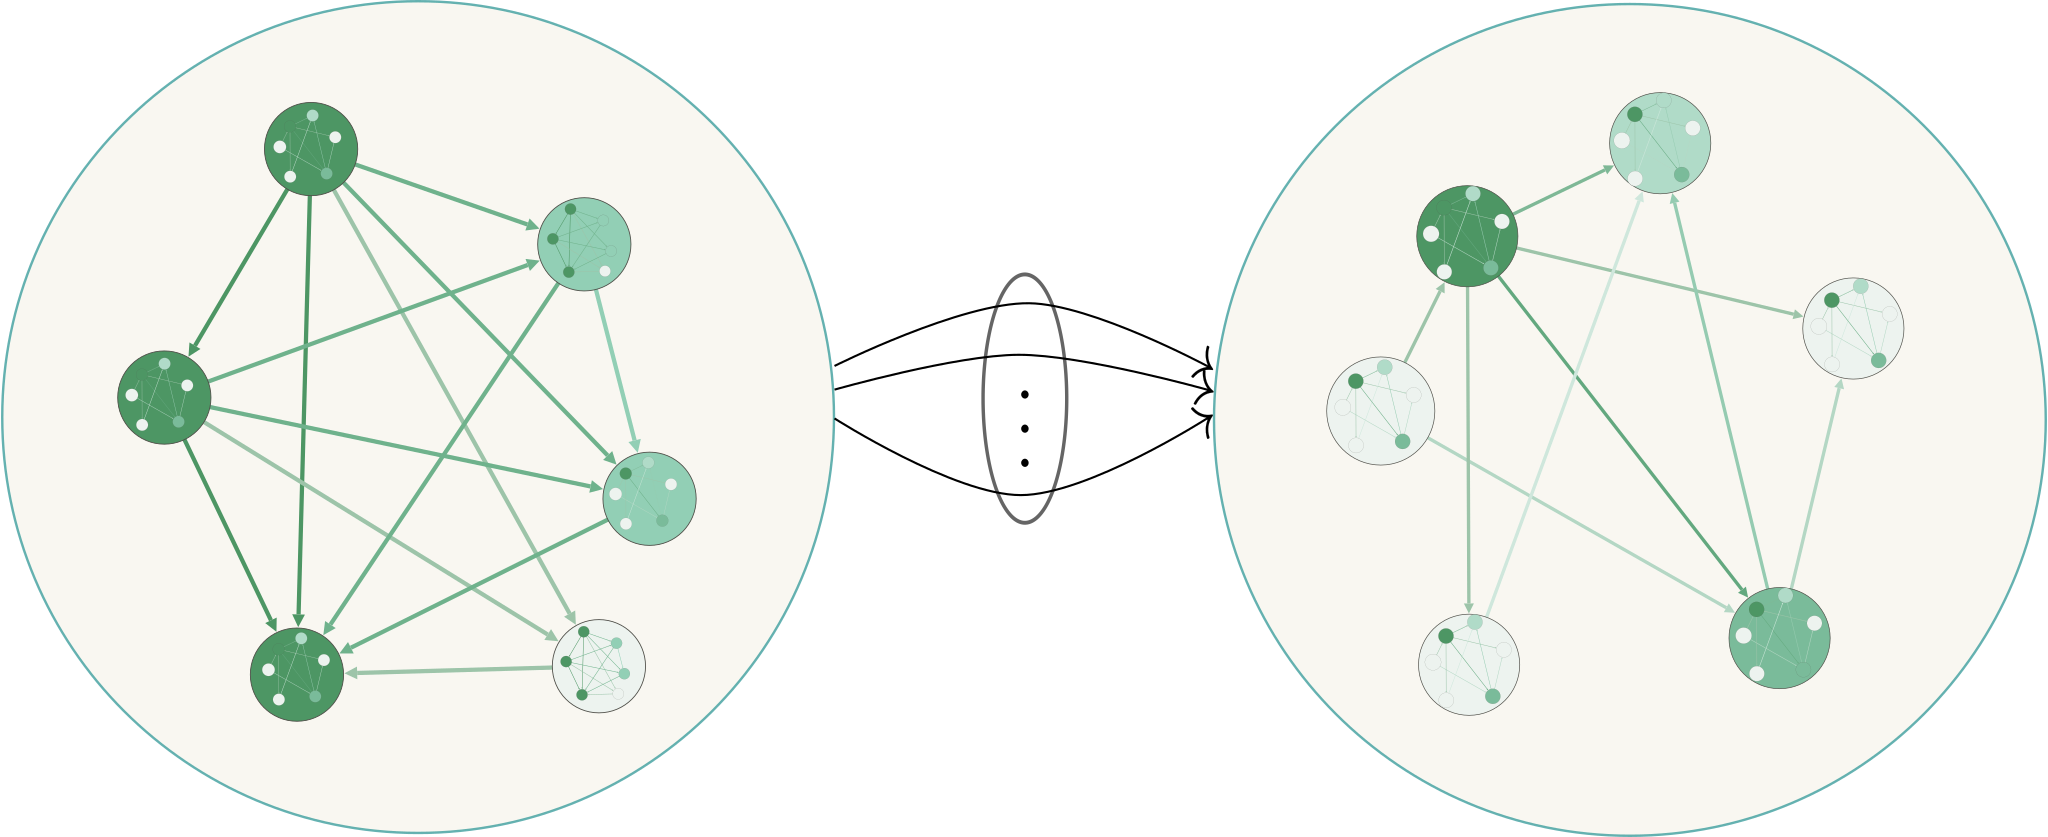
\includegraphics[width=1.0\framewidth]{fig/biograph.pdf}
\caption{%Particular features of interaction networks underlying biological systems can be abstracted as algebraic structures of some type with morphisms translating structure between them. 
On the left is a representation of the integrated metabolic-gene regulatory glycolytic network of E. coli K12 MG1655 derived from the EcoCyc database \cite{Keseler2011} in terms of the BioPAX ontology \cite{Demir2010}. 
%On the right is a conceptual picture of the way in which the relationships between substructure of a particular network can be represented algebraically in terms of algebraic structures that can be referred to as objects and methods of transforming or mapping between these structures referred to as morphisms.}
}
\label{fig:biograph}
\end{figure}
\end{frame}

\begin{frame}
\begin{quotation}
{\it One [...] idea, which underlies everything in this book, is the concept
of genomically encoded information processing. [...],
this is like the geological basis of the landscape. In my view, cis-regulatory information processing, and information processing at the gene regulatory network circuit level, are the real secret of animal development. Probably the appearance of genomic regulatory systems capable of information processing is what made animal evolution possible.} -Eric H. Davidson \cite{Davidson2006a}
\end{quotation}
\end{frame}

\begin{frame}
\begin{enumerate}
\item The development of a formal language for modeling and reasoning about biological systems was suggested by Joseph Woodger in collaboration with the developmental biologist Conrad Waddington and the logician Alfred Tarski as early as 1937 \cite{Woodger1937,Woodger1951,Woodger1952,Woodger1952a}. 
\item At that time it was perhaps difficult to understand how such a language could be put to use. 
\item Today we have tools that could enable the use of such a language:
\begin{enumerate}
\item computational machines to automate the details of routine transformations within the language 
\item accessible, growing repositories of biological data.
\end{enumerate} 
\end{enumerate}
\end{frame}

\begin{frame}
\begin{enumerate}
\item Category theory \cite{Lane1985,Lane1998,MacLane1992,Lawvere1997,Lawvere2003,Awodey2006} is a language that has been suggested since Woodger to provide a framework for representing and reasoning about biological systems \cite{Rashevsky1954,Rosen1958,Rosen1958a,Rosen1978,GOGUEN1979,Rosen1985,Rosen1991,Ehresmann2007,Louie2009} 
\item What is immediately useful about this language from the perspective of biology and its underlying chemistry is that it presents as primitive the notion of transformation between objects. 
\item From this point of view, a defining characteristic of any representation of an entity (e.g. a protein, cell, organism, or population) is the set of relationships between its representations of other entities under consideration. 
\item Intrinsic properties are taken into account implicitly in this framework since the possible set of relationships between any object and any other is constrained by the nature of its intrinsic properties. 
\end{enumerate}
\end{frame}

\begin{frame}
\begin{figure}
\noindent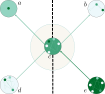
\includegraphics[width=0.5\framewidth]{fig/infopres.pdf}
\caption{%Particular features of interaction networks underlying biological systems can be abstracted as algebraic structures of some type with morphisms translating structure between them. 
From bottom to top and on the left we imagine an information non-preserving interaction resulting from the inability of $a$ to distinguish the interaction of $d$  with $c$ from that of $e$ with $c$, whereas on the right we imagine an information preserving interaction wherein $b$ is capable of distinguishing the interaction of $d$  with $c$ from that of $e$ with $c$.
%On the right is a conceptual picture of the way in which the relationships between substructure of a particular network can be represented algebraically in terms of algebraic structures that can be referred to as objects and methods of transforming or mapping between these structures referred to as morphisms.}
}
\label{fig:infopres}
\end{figure}
\end{frame}